%\sub
\seccion{Variedad Diferenciable}
\label{s:WL:VariedadDiferenciable}

Sobre una  variedad topol\'ogica  se puede ``montar''  una nueva  estructura. Es
posible  hacer  eso imponiendo  condiciones  de  diferenciabilidad  a los  mapas
coordenados de  la definici\'on  de una variedad  topol\'ogica. Sin  embargo, no
tenemos   definida  la   noci\'on   de  diferenciablidad   sobre  una   variedad
cualquiera.  Por  ello, para  definir  una  estructura  diferenciable sobre  una
variedad  topol\'ogica  arbitraria,  recurrimos  a  $\Rset^n$  donde  si  est\'a
definida la noci\'on de diferenciabilidad. Por ello hacemos la siguiente:
%
\begin{definicion}[$C^r$-compatibilidad]
  Diremos que dos cartas coordenadas  $(U,\phi)$ y $(V,\psi)$ sobre una variedad
  $\M$ son  $C^r$-compatibles si  cuando $U \bigcap  V \ne \emptyset  $ entonces
  $\phi \circ \psi^{-1}$  y $\psi \circ \phi^{-1}$ son de  clase $C^r$ sobre los
  subconjuntos  $\phi(U  \bigcap  V)$   y  $\psi(U  \bigcap  V)$  de  $\Rset^n$,
  respectivamente.
\end{definicion}
%
Con esto podemos avanzar en la siguiente:
%
\begin{definicion}[Variedad diferenciable]
  Una {\it Variedad diferenciable} $n$-dimensional  de clase $C^r$, $\M$, es una
  variedad  topol\'ogica  y una  familia  de  cartas  coordenadas $\B  =  \left(
    U_\alpha , \phi_\alpha \right)$, tales que:
  %
  \begin{enumerate}
  \item los $U_{\alpha}$ cubren $\M$,
  %
  \item  para cualquier  par $\alpha,  \beta$, los  entornos $\left(  U_\alpha ,
      \phi_\alpha \right)$  y $\left( U_\beta  , \phi_\beta \right)$  son $C^r$-
    compatibles,
  %
  \item  Cualquier   entorno  coordenado  $(V,\psi)   \:\:  C^r$-compatible  con
    cualquiera de los  $\left( U_\alpha , \phi_\alpha \right)  \in \B$ est\'a en
    $\B$.
  \end{enumerate}
\end{definicion}

\begin{figure}
 \centerline{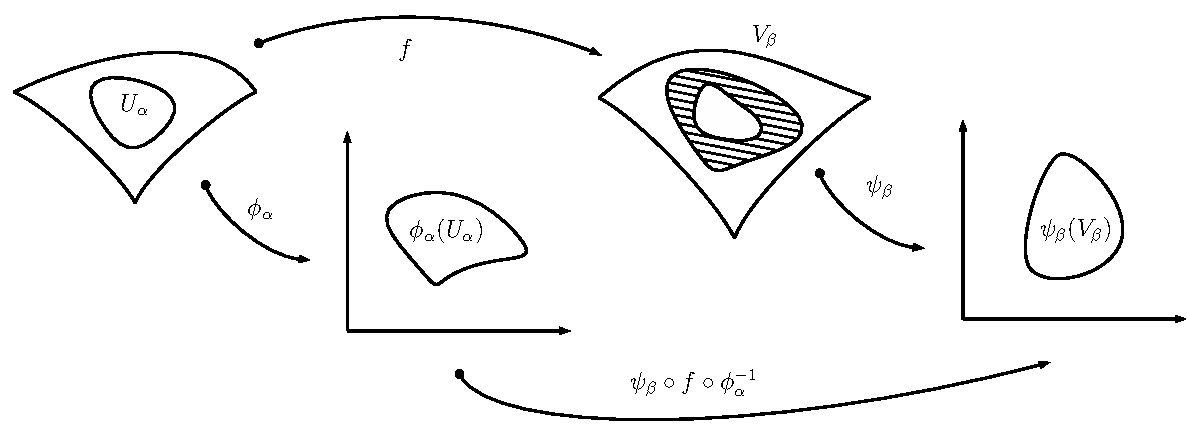
\includegraphics[width=13cm]{figura2.pdf}}
%
 \leyenda{Cartas  coordenadas  usadas  en   la  definici\'on  de  una  funci\'on
   diferenciable.}
\end{figure}

Cualquier  superficie ``suave''  en $\Rset^3$  es un  ejemplo de  (sub) variedad
diferenciable. Este ejemplo no debe conducir  a la confusi\'on de pensar que una
variedad debe estar inmersa en $\Rset^n$. Otro ejemplo de variedad diferenciable
de dimensi\'on $n$ es la esfera $\Sset^n$, definida previamente.

\begin{definicion}[Diferenciabilidad de clase $C^k$]
  Dadas  dos variedades  $\M$ y  $\M'$ de  clase $C^r$,  una  aplicaci\'on $f:\M
  \rightarrow \M' $,  se dice {\it diferenciable} de clase $C^k,  \quad k \le r$
  si para  toda carta  $\left( U_\alpha  , \phi_\alpha \right)$  de $\M$  y toda
  carta  de $\left(  V_\beta ,  \psi_\beta \right)$  de $\M'$  tal  que $f\left(
    U_\alpha \right) \subset V_\beta$, la aplicaci\'on $\psi_\beta \circ f \circ
  \phi_\alpha^{-1}$ de $\phi_\alpha\left( U_\alpha \right)$ en $\psi_\beta\left(
    V_\beta \right)$, es diferenciable de clase $C^k$.
\end{definicion}

El disponer  de la noci\'on de  funci\'on diferenciable, permite  asignar a cada
punto de una variedad diferenciable,  un espacio vectorial. \'Este estar\'a dado
por operadores  lineales que act\'uan  sobre funciones diferenciables y  dan por
resultado un n\'umero.  Antes de ir a la definici\'on  de ese espacio vectorial,
introducimos el concepto de curva suave sobre una variedad.
%
\begin{definicion}[Curva de clase $C^k$ sobre una variedad]
  Sea $\M$  una variedad de  clase $C^r$. Una  curva $\lambda$ en $\M$  de clase
  $C^k, \quad k  \le r$ es una funci\'on  del intervalo real $[a \, ,  \, b]$ en
  $\M$ tal que  para toda carta $\left( U_\alpha ,  \phi_\alpha \right)$ en $\M$
  la composici\'on
  %
  \[
  \phi_\alpha \circ \gamma: [a \, , \, b] \rightarrow \phi_\alpha\left( U_\alpha
  \right)
  \]
  %
  es de clase $C^k$. En coordenadas
  %
  \[
  \phi_\alpha \circ \gamma (t) = \{ x^1(t) , \ldots , x^n(t) \}
  \]
\end{definicion}
%
Con esto podemos ahora dar la noci\'on de vector tangente a una variedad:
%
\begin{definicion}[Tangente a una variedad]
  Sea $\F(p)$ el  conjunto de funciones diferenciables de  clase $C^1$ definidas
  en un entorno del punto $p$.  Sea $\gamma(t)$ una curva de clase $C^1$, $a \le
  t  \le b$  tal que  $\gamma(t_0) =  p$. El  vector {\it  tangente} a  la curva
  $\gamma(t)$ en el punto $p$ es una aplicaci\'on $\mathbb{X}_p : \F(p) \rightarrow \Rset$
  % \[
  % \mathbb{X}_p : \F(p) \rightarrow \Rset
  % \]
  cuyo efecto es
  %
  \[
  \mathbb{X}_p f = \frac{df(\gamma (t))}{dt} |_{t_0}
  \]
\end{definicion}
%
El vector $\mathbb{X}_p$ satisface las siguientes propiedades
%
\begin{itemize}
 \item $\mathbb{X}_p$ es una aplicaci\'on lineal de $\F(p)$ en $\Rset$,
  %
 \item  $\mathbb{X}_p(fg) =  \left( \mathbb{X}_p  f \right)  g(p) +  f(p) \left(
     \mathbb{X}_p g \right)$ para $f , g \in \F(p)$.
\end{itemize}
%
Dejamos para el lector demostrar estas propiedades.

Sean $(u^1 , \ldots  , u^n)$ coordenadas locales en un entorno  $U$ de $p$. Para
cada $j$, $\left( \frac{\partial}{\partial  u^j} \right)|_p$ es una aplicaci\'on
de $\F(p)$  en $\Rset$ la cual satisface  las propiedades (i) e  (ii). Veremos a
continuaci\'on que el conjunto de todas las aplicaciones $\mathbb{X}$ de $\F(p)$
en $\Rset$ es un espacio vectorial $n$-dimensional, siendo $n$ la dimensi\'on de
la variedad diferenciable $\M$.

Dada una  curva $\gamma(t)$ con $\gamma(t_0)  = p$, sean  $u^j(t) = \gamma^j(t),
\quad  j =  1 ,  \ldots ,  n$  las coordenadas  locales de  esa curva.  Entonces
$\frac{df(\gamma(t))}{dt}|_{t_0}  =  \sum_j  \left(  \frac{\partial  f}{\partial
    u^j}|_p  \right)  \left( \frac{d  \gamma^j  (t)}{dt} \right)|_{t_0}$.  Extra %% ESTA???
expresi\'on indica  que todo vector  en $p$ es  una combinaci\'on lineal  de los
vectores (operadores).

\begin{equation}
\left(\frac{\partial}{\partial u^1}|_p \right),\ldots,\left(\frac{\partial}{\partial u^n}|_p \right) \label{set}
\end{equation}

Sea la  combinaci\'on lineal  $\sum_j \xi^j \frac{\partial}{\partial  u^j}|_p$ y
sea la curva definida por
%
\[
u^j(t) = u^j(p) + \xi^j t \quad j = 1 , \ldots , n
\]
%
El   vector   tangente   a   esta   curva   en  $t   =   0$   es   $\sum   \xi^j
\frac{\partial}{\partial u^j}|_p$.  Adem\'as si
%
\[
\sum \xi^j \frac{\partial}{\partial u^j}|_p =0,
\]
%
entonces
%
\[
0 = \sum \xi^j \left( \frac{\partial u^k}{\partial u^j} \right)|_p = \xi^k \quad
k = 1 , \ldots , n
\]
%
Esto demuestra la independencia lineal de los vectores~\eqref{set}.
%
\begin{definicion}[Espacio tangente]
  El conjunto  de vectores tangentes en $p  \in \M$, es llamado  el {\it espacio
    tangente de $\M$ en $p$}, y lo denotaremos por $T_p(\M)$.
\end{definicion}

La colecci\'on de todos los  espacios tangentes, $\bigcup_{p \in \M} T_p(\M)$ se
llama {\it fibrado tangente}.

Al fibrado tangente se le puede  dar la estructura de un \'algebra (\'algebra de
Lie). Esta surge de calcular  el conmutador $[\mathbb{X}, \mathbb{Y}]$ entre dos
campos vectoriales $\mathbb{X}$ e $\mathbb{Y}$:
%
\[
[\mathbb{X},  \mathbb{Y}] f  \equiv  \left( \mathbb{X}  \mathbb{Y} -  \mathbb{Y}
  \mathbb{X} \right) f
\]
%
Si los vectores  se escriben en t\'ermino de los vectores  de la base coordenada
$\left(  \frac{\partial}{\partial  x^a}  \right)$,  el  conmutador  entre  ellos
resulta ser el vector:
%
\[
\sum_{ab} X^a \frac{\partial  Y^b}{\partial x^a} \frac{\partial}{\partial x^b} -
\sum_{ab} Y^a \frac{\partial X^b}{\partial x^a} \frac{\partial}{\partial x^b}
\]

A cada espacio tangente $T_p(\M)$ podemos asignar su dual, $T_p^*(\M)$, es decir
el conjunto de  todos los operadores lineales y  homog\'eneos que act\'uan sobre
$T_p(\M)$.   A    un   elemento   del   espacio   dual    lo   llamaremos   {\it
  $1$-forma}. Denotaremos a  la acci\'on de un elemento  de $T_p^*(\M)$, digamos
$\omega_p$, por:
%
\[
\omega_p(\mathbb{X}_p) = \left\langle \omega_p , \mathbb{X}_p \right\rangle.
\]
%
Para cada  funci\'on $f \in  \F(p)$, el {\it  diferencial de $f$},  denotado por
$(df)_p$, es el elemento de $T_p^*(\M)$ que tiene por acci\'on:
%
\[
\left\langle (df)_p ,  \mathbb{X}_p \right\rangle = \mathbb{X}_p f,  \quad \mathbb{X}_p \in
T_p(\M)
\]

Cada funci\'on coordenada $u^j$ es una funci\'on de $\M$ sobre $\Rset$. Entonces
podemos  calcular  el  diferencial  de  $u^j$, cuya  acci\'on  sobre  un  vector
$\mathbb{X}_p \in T_p(\M)$ est\'a dada por
%
\[
 \left\langle (du^j)_p , \mathbb{X}_p \right\rangle = \mathbb{X}_p^j
\]
%
En particular,  si $\mathbb{X}_p =  \left(\frac{\partial}{\partial u^k} \right)$
resulta
%
\[
\left\langle   (du^j)_p   ,   \left(   \frac{\partial}{\partial   u^k}   \right)
\right\rangle = \delta_k^j;
 \]
%
 es decir $\left\{ (du^j)_p \right\}_{j=1}^n$ es la base dual de $\left\{ \left(
     \frac{\partial}{\partial  u^j} \right)_p \right\}_{j=1}^n$.  Toda $1$-forma
 $\omega$ se puede escribir en t\'ermino de esta base:
%
\[
\omega = \sum_a \omega_a dx^a
\]

Con los espacios  $T_p(\M)$ y $T_p^*(\M)$ podemos construir  el espacio producto
cartesiano
%
\[
\left(  T_p(\M)  \right)_s^r =  T_p(\M)  \times  T_p(\M)  \ldots T_p(\M)  \times
T_p^*(\M) \times T_p^*(\M) \ldots \times T_p^*(\M)
\]
%
con $r$ factores de $T_p(\M)$ y $s$ factores de $T_p^*(\M)$.

\begin{definicion}[Tensor de tipo $(r,s)$]
  Un {\it tensor de tipo $(r,s)$} es un operador $S$,
  %
  \[
  S: \left( T_p(\M) \right)_s^r \rightarrow \Rset
  \]
  %
  que es lineal y homog\'eneo en cada uno de sus argumentos.
\end{definicion}

\begin{definicion}[Campo tensorial]
  Un {\it campo tensorial $S$ de  clase $C^k$ de tipo $(r,s)$ sobre $V \subseteq
    \M$} es un mapa  $C^k$ que asigna un tensor de tipo  $(r,s)$ a cada punto $p
  \in V$.
\end{definicion}
%
En  t\'ermino  de las  bases  $\left\{  \left( \frac{\partial}{\partial  u^j}|_p
  \right)  \right\}_{j=1}^n$  y $\left\{  (du^j)_p  \right\}_{j=1}^n$, el  campo
tensorial $S$ se puede escribir:
%
\[
S(p) = S^{a_1 \ldots  a_r}_{b_1 \ldots b_s}(p) \frac{\partial}{\partial x^{a_1}}
\bigotimes   \ldots  \bigotimes  \frac{\partial}{\partial   x^{a_r}}  \bigotimes
dx^{b_1} \bigotimes \ldots \bigotimes dx^{b_s}
\]
%
\noindent donde  las funciones $S^{a_1 \ldots a_r}_{b_1 \ldots b_s}$  son de clase
$C^k$ y $\bigotimes$ es el producto tensorial.

Entre los campos tensoriales que se  pueden definir sobre una variedad $\M$, hay
uno particularmente importante,  y es conocido como el  tensor m\'etrico. \'Este
se define por medio de un producto escalar:
%
\begin{definicion}[Producto escalar]
  Un {\bf producto escalar} sobre $T_p(\M)$ es una funci\'on
  %
  \[
  g: T_p(\M) \times T_p(\M) \rightarrow \Rset
  \]
  %
  que satisface
  %
  \begin{enumerate}
  \item $g(\mathbb{X}, \mathbb{Y}) = g(\mathbb{Y}, \mathbb{X}), \quad \text{para}
    \quad \mathbb{X}, \mathbb{Y} \in T_p(\M)$
  %
  \item  $g(\mathbb{X},   a  \mathbb{Y}  +  b  \mathbb{Z})   =  a  g(\mathbb{X},
    \mathbb{Y}) + b g(\mathbb{X}, \mathbb{Z})$
  \end{enumerate}
\end{definicion}

El producto escalar se dice  {\it no degenerado} si $g(\mathbb{X}, \mathbb{Y})=0
\quad \forall \:  \mathbb{Y} \in T_p(\M)$ implica $\mathbb{X}  = 0$.  Obviamente
el  producto  escalar  es un  tensor  de  tipo  $(0,2)$.  Como  campo  tensorial
$g(\;,\;)$   se   puede   expresar    en   t\'erminos   de   la   base   $\left(
  \frac{\partial}{\partial    u^1}|_p     \right)    ,    \ldots     ,    \left(
  \frac{\partial}{\partial u^n}|_p \right)$
%
\[
g(\mathbb{X}, \mathbb{Y})  = \sum_{ab} X^a  Y^b g\left( \frac{\partial}{\partial
    u^a}, \frac{\partial}{\partial u^b} \right)
\]
%
o, de manera equivalente
%
\[
g(\mathbb{X}, \mathbb{Y}) = \sum_{ab} g_{ab} X^a Y^b
\]
%
donde     $g_{ab}    =    g     \left(    \frac{\partial}{\partial     u^a}    ,
  \frac{\partial}{\partial  u^b}   \right)$.  Si  el  producto   escalar  es  no
degenerado, entonces  existe la  matriz inversa de  la matriz $g_{ab}$,  a cuyos
elementos los denotaremos por $g^{ab}$, de modo que
%
\[
\sum_c g_{ac} g^{cb} = \delta_a^b
\]

La  existencia de  un campo  tensorial  m\'etrico (o  producto escalar  definido
localmente),  permite introducir  la idea  de {\it  longitud de  una  curva}. En
efecto, sea  $\gamma(t), \quad t  \in [a \,  , \, b]$  una curva de  clase $C^1$
sobre $\M$,  que une los  puntos $p$  y $q$: $\gamma(a)  = p, \quad  \gamma(b) =
q$. En el punto $\gamma(t)$ tenemos  el vector tangente a la curva $\gamma$ dado
por
%
\[
\left( \frac{\partial}{\partial t} \right)_\gamma = \sum_j \frac{d \gamma^j}{dt}
\frac{\partial}{\partial x^j}
\]

\begin{definicion}[Longitud de una curva]
  La {\it longitud de la curva $\gamma$  entre los puntos $p$ y $q$} est\'a dada
  por la cantidad
  %
  \begin{equation}
    L = \int_a^b | g \left( \frac{\partial}{\partial t}, \frac{\partial}{\partial t} \right) |^{\frac{1}{2}} dt
  \label{longitud}
  \end{equation}
\end{definicion}
%
O, equivalentemente
%
\begin{equation}
L = \int_a^b \left| \sum_{ij} g_{ij}(x) \frac{d\gamma^i}{dt} \frac{d \gamma^j
}{dt} \right|^{\frac{1}{2}} dt \label{longitud}
\end{equation}